\chapter{Área de estudo}\label{cap:area-estudo}

A Bacia de Santos é uma bacia sedimentar de margem passiva localizada no Atlântico Sul Ocidental, entre os altos de Cabo Frio, ao norte, e de Florianópolis, ao sul. Ocupa aproximadamente 350.000 km² até a isóbata de 3.000 m e abrange a margem sudeste brasileira, desde o litoral do Rio de Janeiro até Santa Catarina \cite{moreira2007}. Sua origem está associada ao rifteamento e à posterior separação entre as placas Sul-Americana e Africana durante o Cretáceo Inferior, processo que condicionou a arquitetura tectonoestratigráfica e a expressiva espessura sedimentar da bacia \cite{macedo1989,moreira2007}.   A região de estudo apresenta gatilhos significativos para a ocorrência de depósitos de movimentos de massa, tais como a sismicidade relacionada à abertura do Atlântico, reativações neotectônicas, tectônica salífera e dissociação de gás \cite{borges2015}. Além disso, outros mecanismos disparadores de movimentos de massa em margens continentais são a presença de ondas internas e de correntes de fundo vinculadas à circulação oceânica \cite{hampton1996}.

Este trabalho concentra-se na porção norte do talude da Bacia de Santos, próxima aos campos de Búzios e Mero (Figura~\ref{fig:localizacao-area-estudo}), entre cotas batimétricas de 800 e 2.000~m. A área é caracterizada por relevo submarino complexo, intensa deformação relacionada à mobilidade do sal aptiano e sucessões sedimentares profundas \cite{moreira2007}. Esses controles estruturais e sedimentares são particularmente relevantes para a investigação de depósitos de transporte de massa (MTDs), pois influenciam os gradientes do substrato, a compartimentação de minibacias e a distribuição de superfícies potencialmente instáveis.

\begin{figure}[htbp]
  \centering
  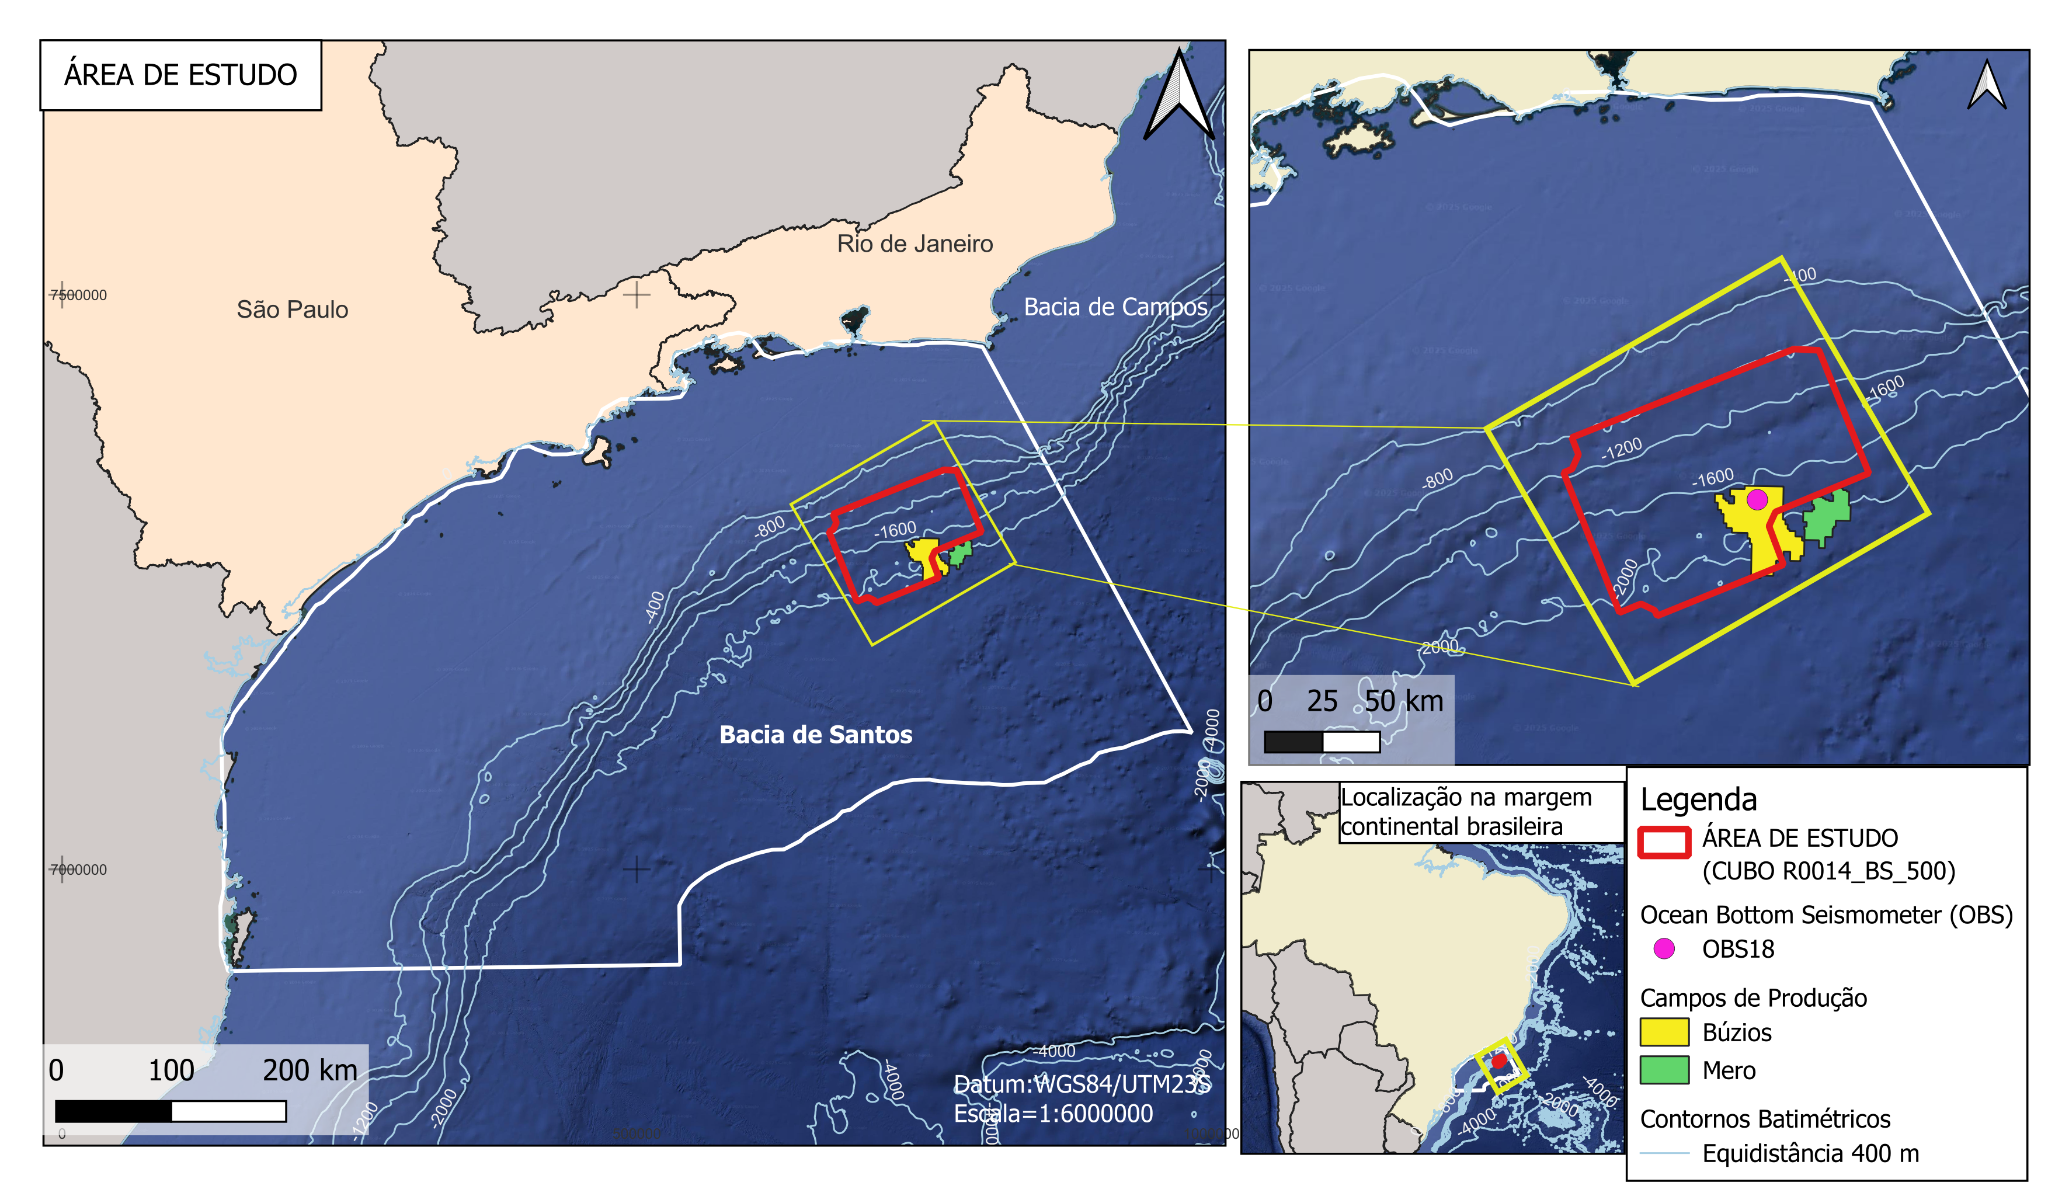
\includegraphics[width=\textwidth,height=0.78\textheight,keepaspectratio]{figuras/area-estudo/figura-17-localizacao-area-estudo.png}
  \caption{Localização da área de estudo. Base de dados: IBGE, ANP e Google Satellite.}
  \label{fig:localizacao-area-estudo}
  \fonte{Elaboração própria.}
\end{figure}

\section{Evolução tectonoestratigráfica}

A evolução da Bacia de Santos está associada à fragmentação do Gondwana e à abertura do Atlântico Sul. As Figuras~\ref{fig:carta-estratigrafica-santos} e~\ref{fig:diagrama-tectonossedimentar-santos} apresentam as principais unidades estratigráficas e sua evolução em relação aos regimes tectônicos. De forma simplificada, o preenchimento compreende os estágios rifte, pós-rifte evaporítico e margem passiva. A fase rifte ocorreu entre o Barremiano e o Eoaptiano, quando a extensão litosférica gerou falhas normais, blocos basculados e depocentros lacustres. Nesse contexto foram depositadas as sucessões pré-sal do Grupo Guaratiba, que incluem rochas vulcânicas, depósitos siliciclásticos e carbonatos lacustres. Essas unidades registram a estruturação inicial da bacia e constituem importantes elementos de seu sistema petrolífero \cite{macedo1989,moreira2007}.

Com o enfraquecimento da tectônica extensional, durante o Aptiano, a bacia passou para uma fase de subsidência predominantemente térmica e restrição progressiva da comunicação com o oceano. Nessa etapa desenvolveu-se um amplo ambiente evaporítico, responsável pela deposição da Formação Ariri. A espessa sequência de sais e evaporitos aptianos representa uma descontinuidade mecânica fundamental na Bacia de Santos: posteriormente, sua baixa densidade e comportamento dúctil permitiram o deslocamento do sal em resposta à sobrecarga sedimentar, à inclinação regional do substrato e às variações de espessura da camada evaporítica. Assim, embora o sal tenha sido depositado durante a fase pós-rifte, sua mobilização controlou grande parte da deformação da seção pós-sal e permanece essencial para interpretar a arquitetura dos depósitos profundos \cite{assine2008,moreira2007}.

A implantação definitiva de condições marinhas ocorreu do Albiano em diante, durante o estágio de margem passiva. Inicialmente, foram depositados os sistemas carbonáticos e siliciclásticos do Grupo Camburi, que inclui as formações Florianópolis, Guarujá e Itanhaém. A Formação Guarujá corresponde a carbonatos de plataforma albiana, enquanto a Formação Itanhaém registra sedimentação marinha mais distal. A partir do Cenomaniano, a movimentação gravitacional do sal e a progradação de cunhas siliciclásticas passaram a gerar expressiva compartimentação do espaço de acomodação. A retirada e o fluxo do sal em direção às regiões distais provocaram \textit{rafting} de pacotes albianos, formação de falhas de crescimento, \textit{rollovers}, muralhas de sal e \textit{minibasins}, especialmente importantes no norte da bacia \cite{assine2008}.

No Cretáceo Superior, os sistemas do Grupo Frade registram o avanço de cunhas terrígenas progradacionais e a instalação de ambientes marinhos profundos. Destacam-se a Formação Itajaí-Açu, predominantemente pelítica, e seu Membro Ilhabela, constituído por arenitos turbidíticos; as formações Santos e Juréia representam, respectivamente, depósitos continentais a costeiros e sedimentos siliciclásticos marinhos de plataforma. A progradação não ocorreu de forma uniforme ao longo da bacia: os depocentros migraram preferencialmente para nordeste, e a porção norte passou a registrar expressivos sistemas deltaicos, turbidíticos e de águas profundas \cite{assine2008}. Esse contexto é diretamente relevante aos MTDs, pois a elevada taxa de aporte sedimentar, o crescimento de clinoformas e a deformação induzida pelo sal favorecem a geração de declives, superfícies de descolamento e irregularidades no relevo do substrato.

Durante o Paleógeno e o Neógeno, a sedimentação passou a ser dominada por depósitos marinhos profundos da Formação Marambaia, associados a sistemas turbidíticos, hemipelágicos e retrabalhados por correntes de fundo. Na plataforma, desenvolveram-se os carbonatos da Formação Iguape, principalmente a partir do Oligoceno, enquanto a Formação Sepetiba reúne os depósitos mais rasos e recentes, de idade quaternária \cite{moreira2007}. Dessa forma, a arquitetura atual da porção norte da Bacia de Santos resulta da interação entre herança rifte, subsidência de margem passiva, progradação siliciclástica, circulação oceânica e tectônica salífera. Essa interação condiciona tanto a distribuição quanto a geometria dos MTDs, que podem ser confinados, desviados ou deformados por estruturas salinas e por minibacias.

\begin{figure}[htbp]
  \centering
  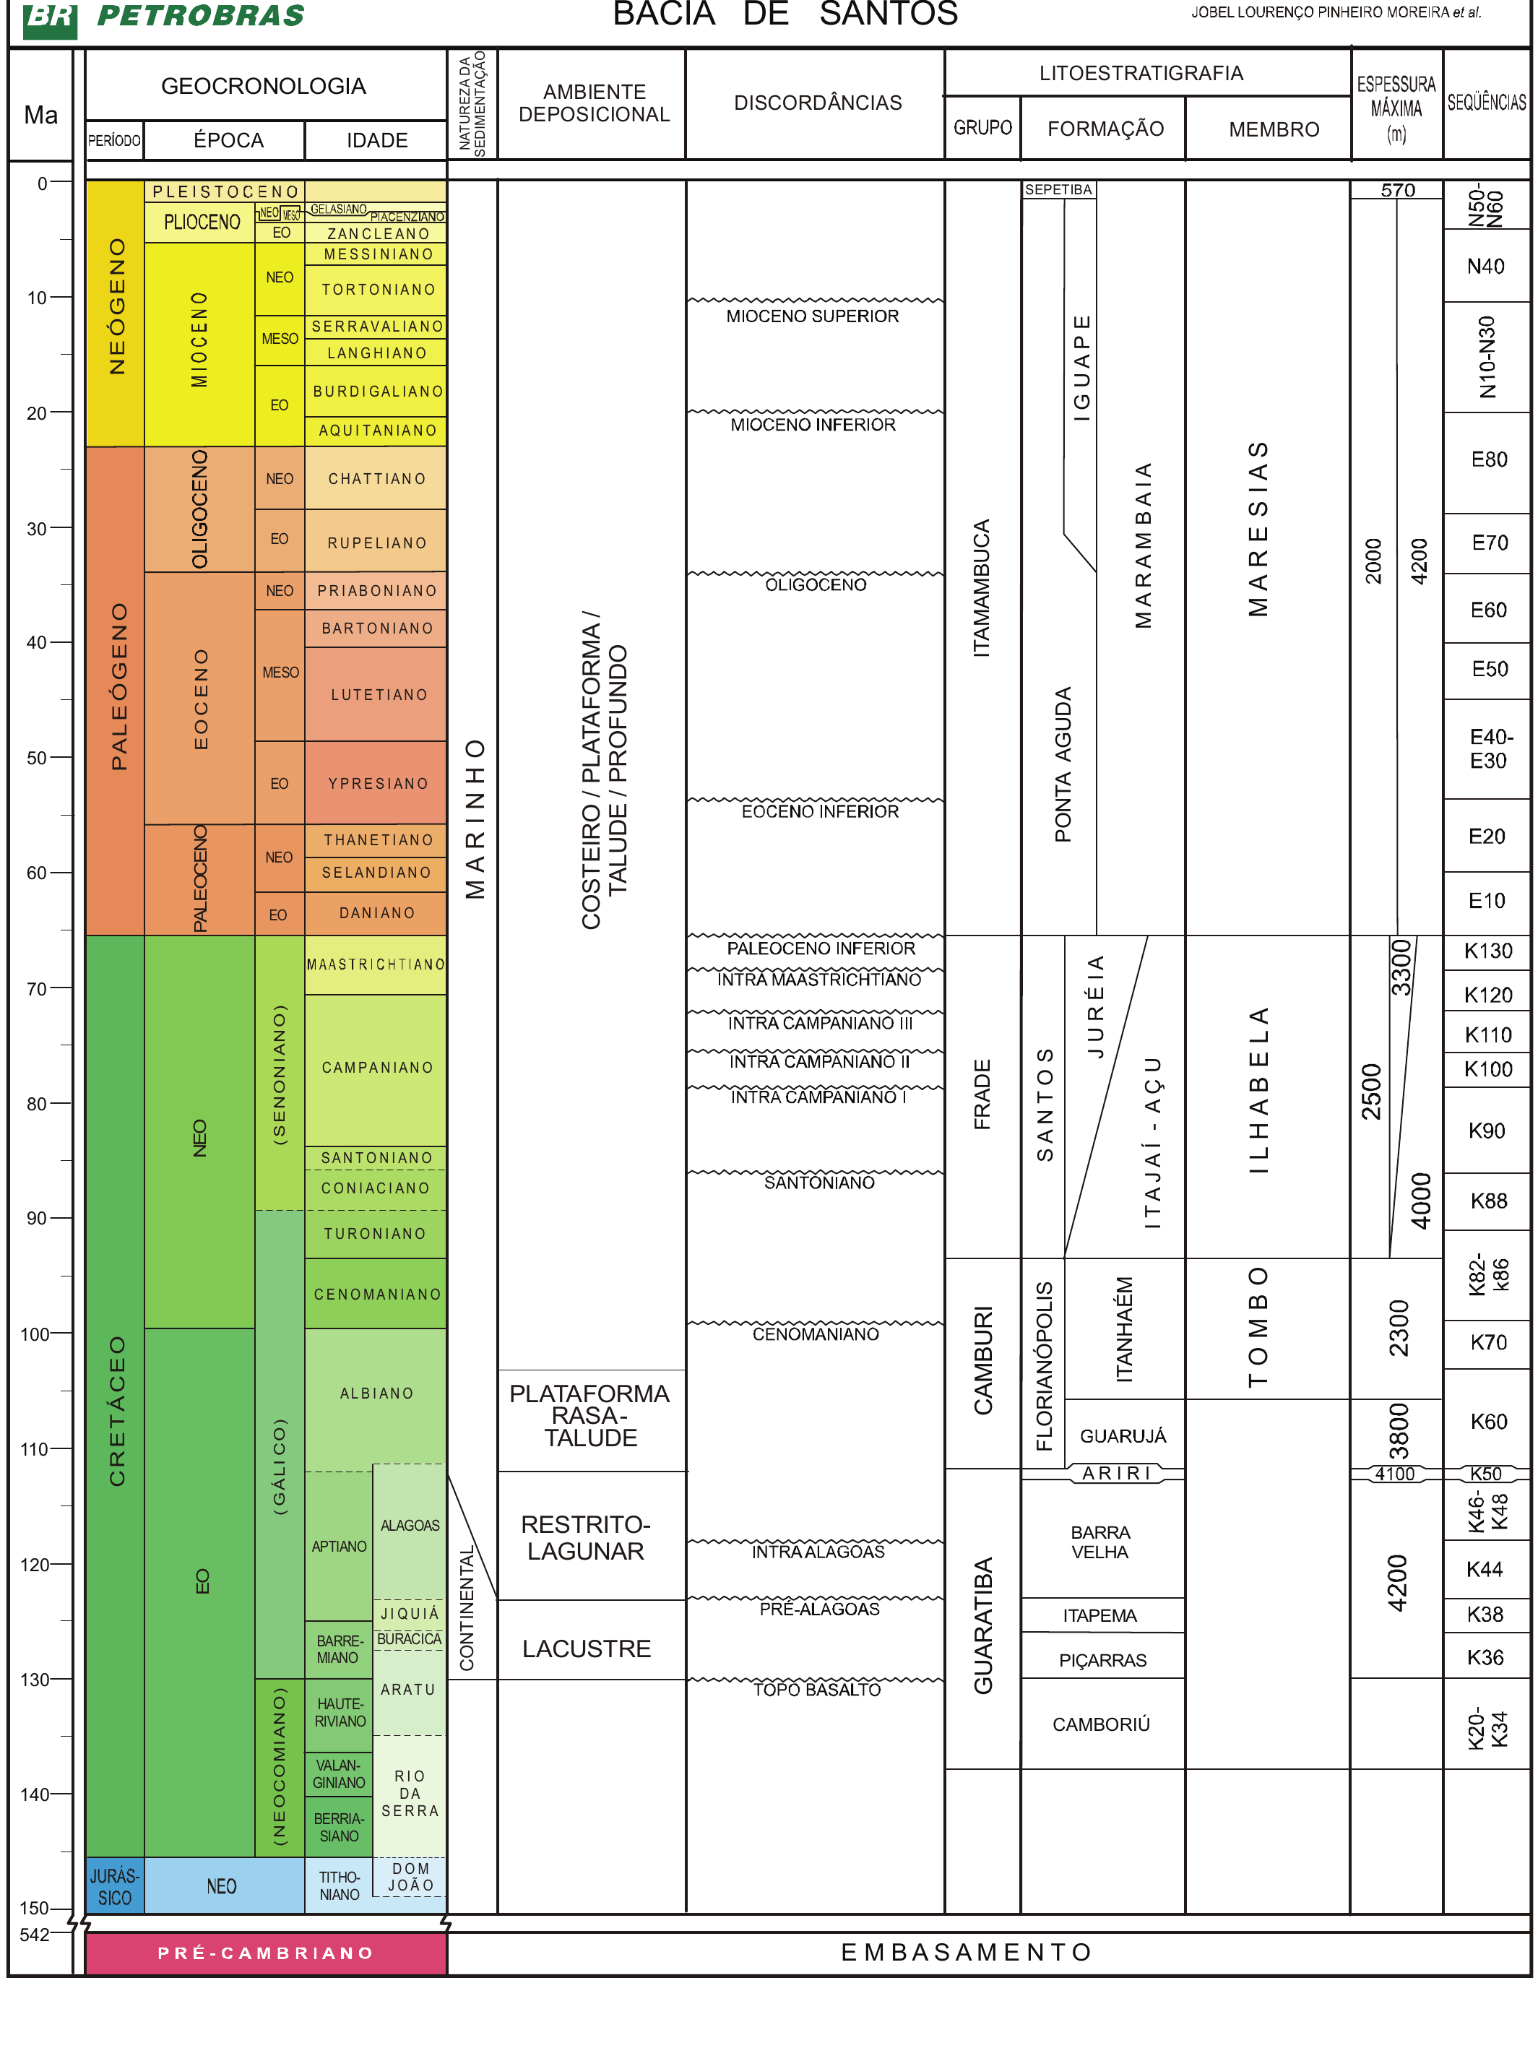
\includegraphics[width=\textwidth,height=0.78\textheight,keepaspectratio]{figuras/area-estudo/figura-17-carta-estratigrafica.png}
  \caption{Carta crono-litoestratigráfica da Bacia de Santos, com destaque para as principais unidades litoestratigráficas, ambientes deposicionais, discordâncias e sequências deposicionais, desde o embasamento pré-cambriano até os depósitos quaternários.}
  \label{fig:carta-estratigrafica-santos}
  \fonte{\citeonline{moreira2007}.}
\end{figure}

\begin{figure}[htbp]
  \centering
  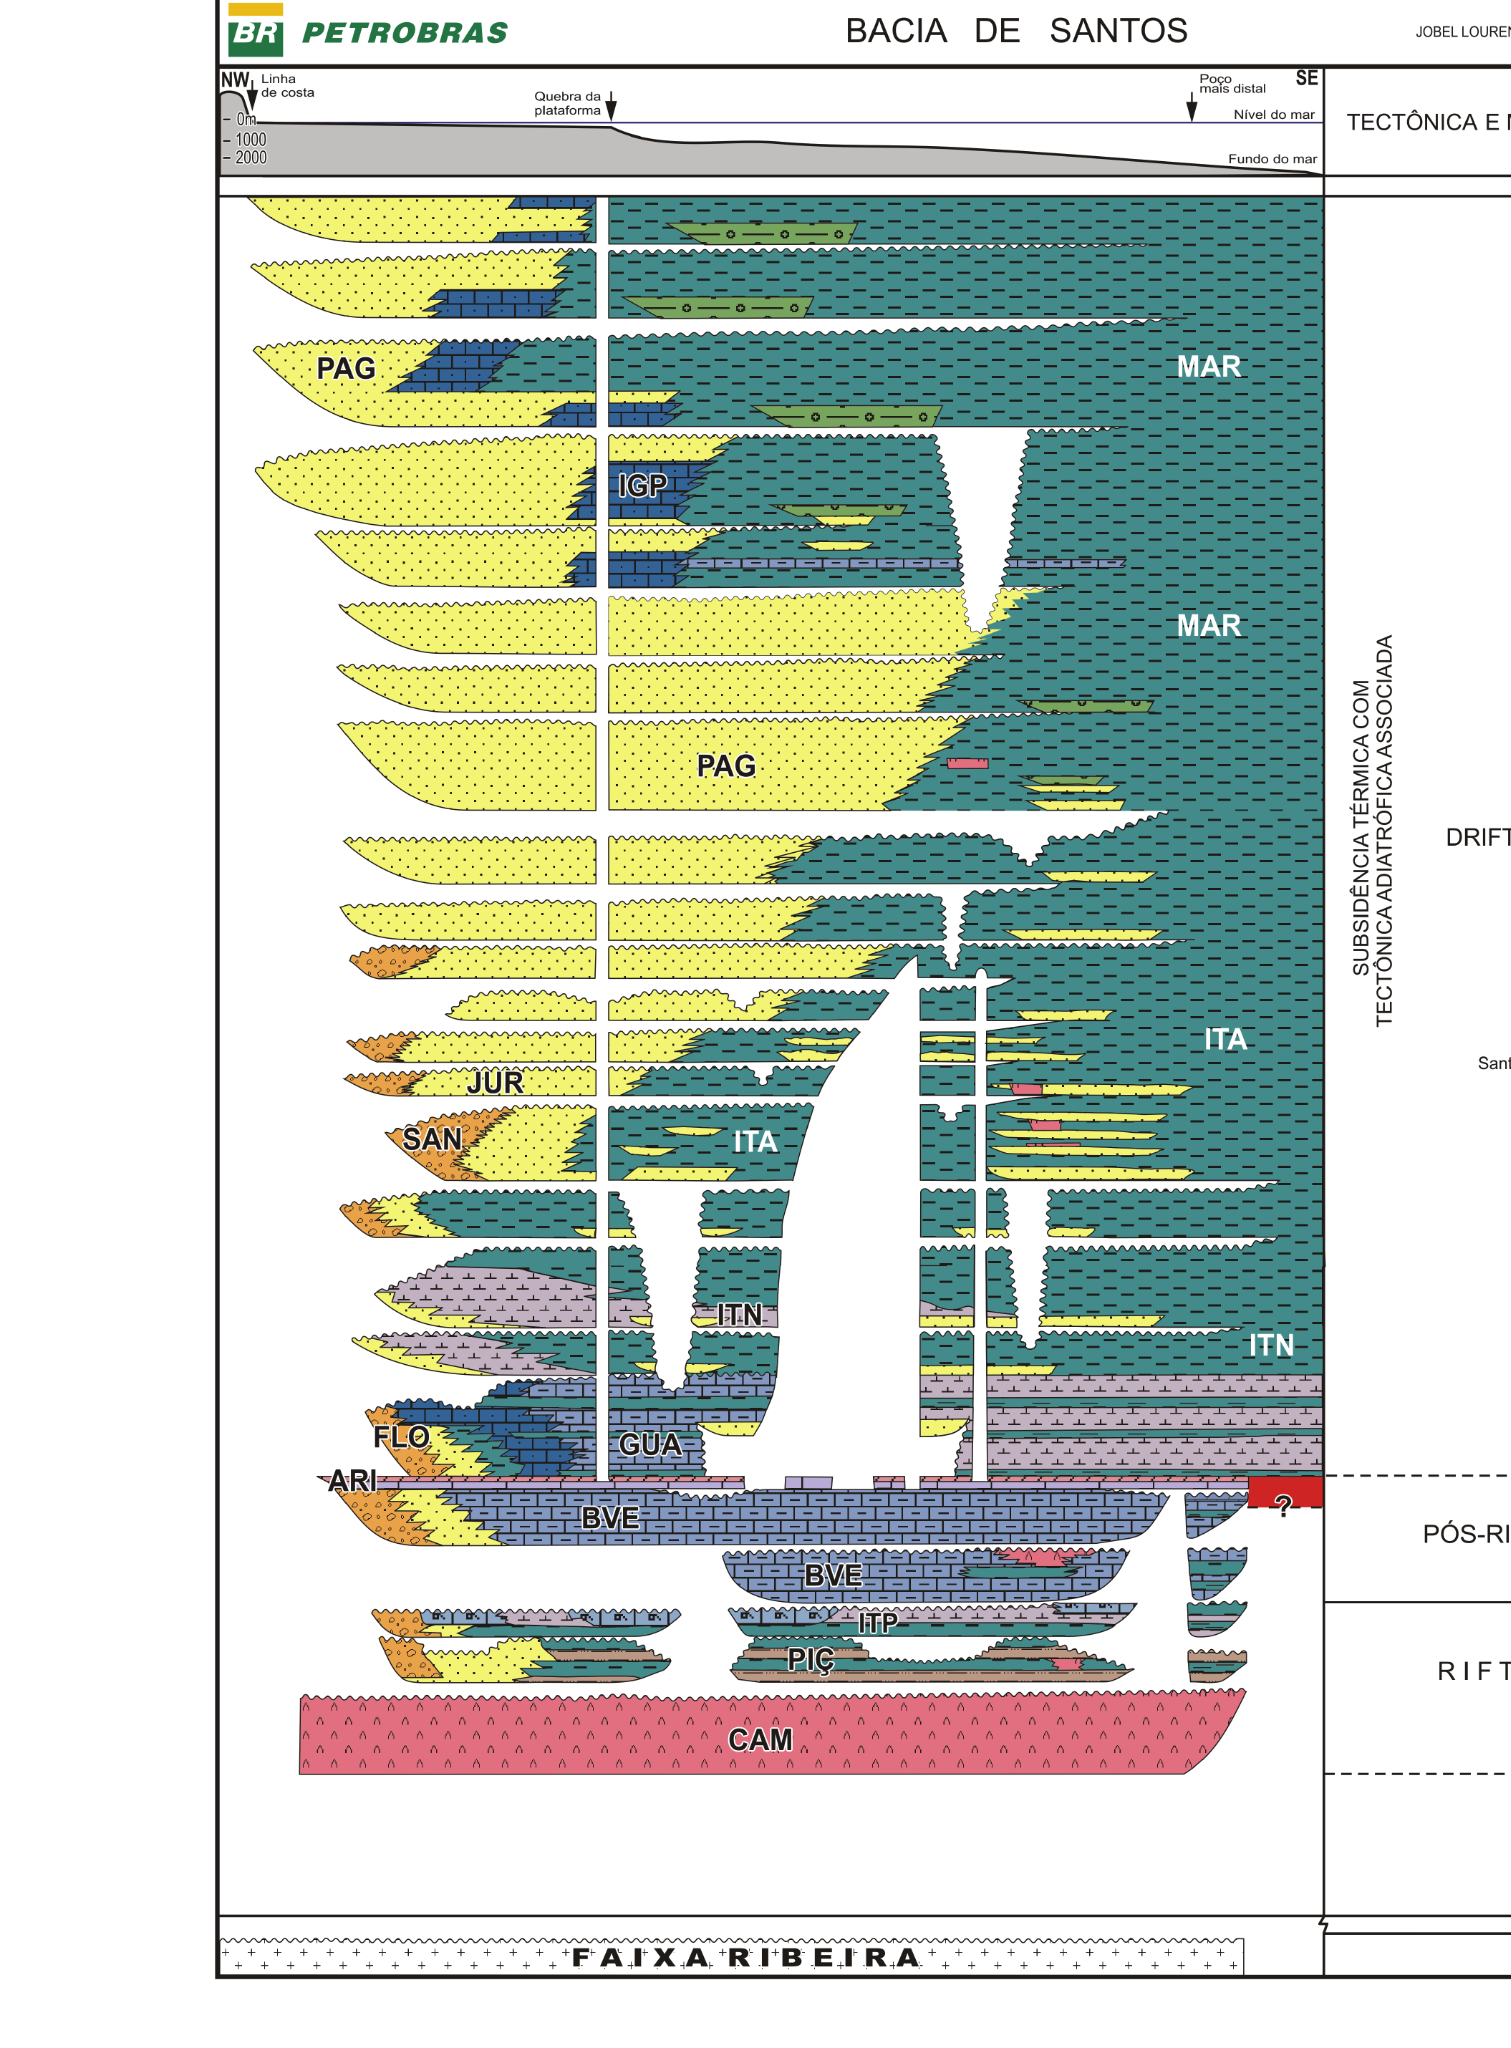
\includegraphics[width=\textwidth,height=0.78\textheight,keepaspectratio]{figuras/area-estudo/figura-18-diagrama-tectonossedimentar.png}
  \caption{Diagrama tectonossedimentar esquemático da Bacia de Santos em seção NW--SE, representando as fases rifte, pós-rifte e drifte, a evolução dos sistemas deposicionais e os principais eventos tectônicos e magmáticos associados ao preenchimento da bacia.}
  \label{fig:diagrama-tectonossedimentar-santos}
  \fonte{\citeonline{moreira2007}.}
\end{figure}

\section{Tectônica salífera e sua influência nos depósitos de transporte de massa}

A tectônica salífera compreende a deformação e a mobilização de evaporitos, principalmente halita, sob condições de carregamento diferencial, gravidade, inclinação regional, heterogeneidades na base do sal e esforços tectônicos. Em escala geológica, o sal apresenta comportamento dúctil e constitui um importante nível de descolamento, capaz de desacoplar parcialmente a cobertura sedimentar de seu substrato. Em margens extensionais, essa propriedade favorece a formação de falhas normais, falhas lístricas, \textit{rollovers}, diápiros, muralhas salinas, almofadas de sal, soldaduras e minibacias \cite{fossen2016,hudec2007,jackson2017} (Figura~\ref{fig:estilos-falhas-sal}).

\begin{figure}[htbp]
  \centering
  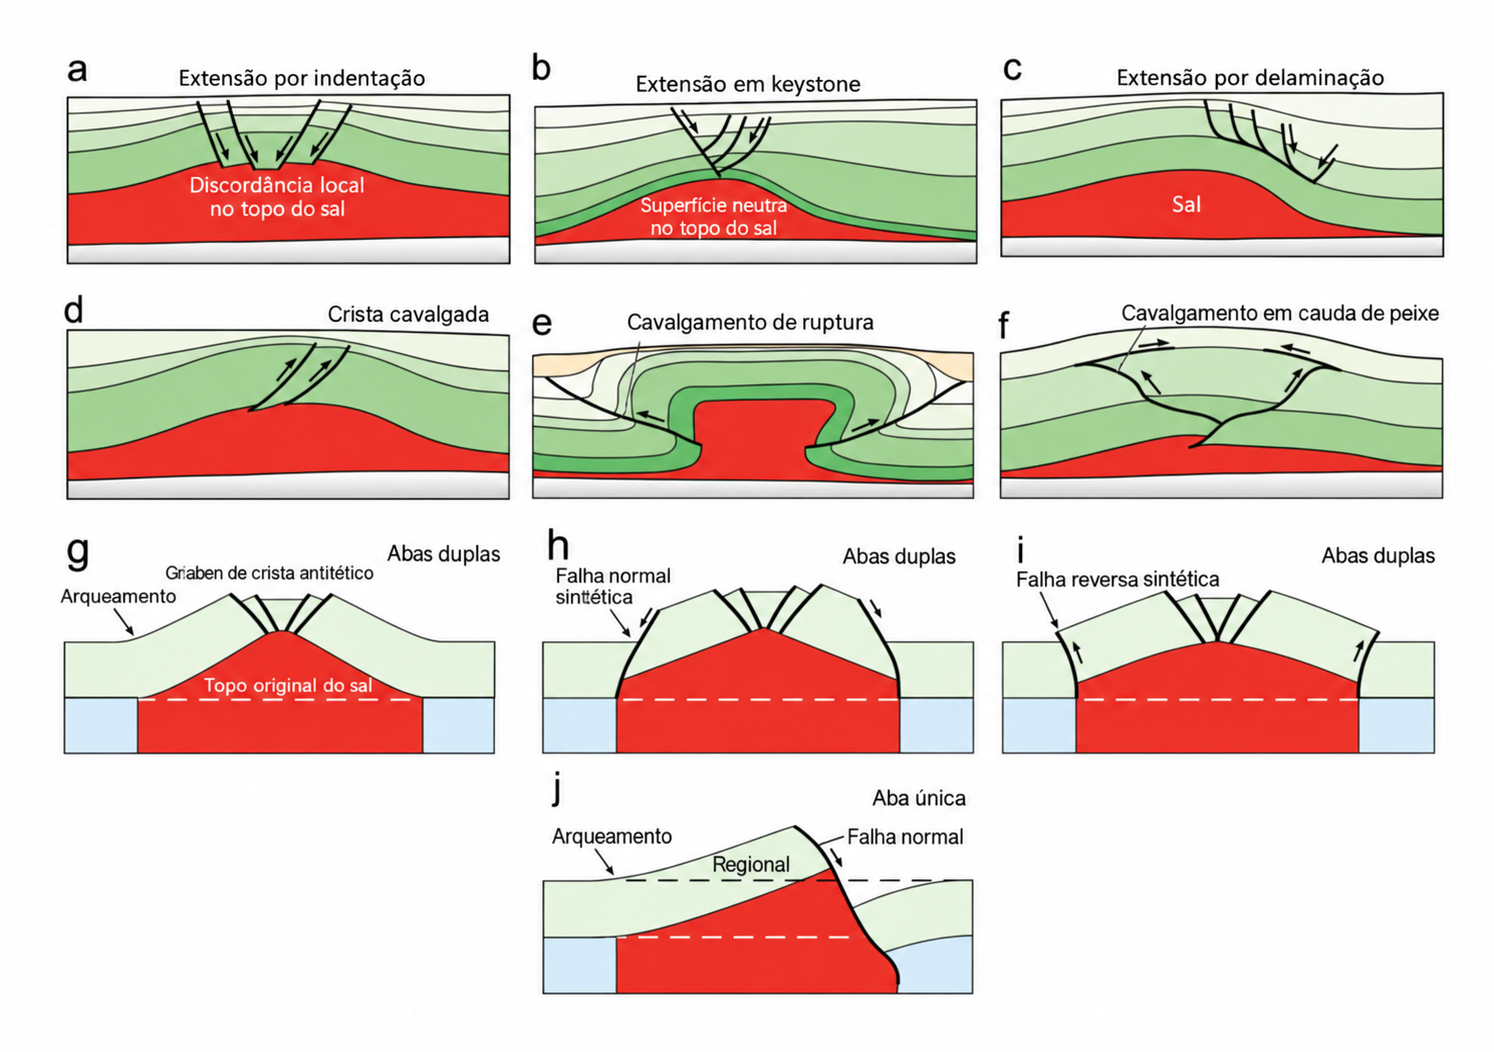
\includegraphics[width=\textwidth,height=0.78\textheight,keepaspectratio]{figuras/area-estudo/figura-19-estilos-falhas-sal.png}
  \caption{Estilos de falhas e deformações associados a anticlinais salinos e cristas salinas. Os painéis a--c representam mecanismos extensionais da cobertura; os painéis d--f, estruturas contracionais; e os painéis g--j, geometrias de falhamento e arqueamento associadas a cristas salinas.}
  \label{fig:estilos-falhas-sal}
  \fonte{Traduzido de \citeonline{jackson2017}.}
\end{figure}

A Bacia de Santos contém uma das mais expressivas províncias evaporíticas do Atlântico Sul, representada pela Formação Ariri, depositada durante o Aptiano. Após a deposição dos evaporitos, a subsidência da margem, a progradação sedimentar e a sobrecarga diferencial promoveram a mobilização do sal em direção às partes mais profundas da bacia. Essa dinâmica resultou em domínios estruturais extensionais, translacionais e contracionais, bem como em significativa deformação da cobertura pós-sal. Na porção norte da Bacia de Santos, a movimentação do sal está relacionada à formação da Falha de Cabo Frio, de muralhas salinas, de diápiros e de minibacias, que controlam a distribuição dos depocentros e a arquitetura estratigráfica das unidades pós-sal \cite{demercian1993,mohriak1995,szatmari1996,assine2008}.

A halocinese não deve ser explicada apenas pela menor densidade do sal em relação às rochas sobrejacentes. A redistribuição dos evaporitos depende da interação entre a geometria da base do sal, a espessura da camada evaporítica, o gradiente regional da bacia, a taxa e a distribuição do aporte sedimentar e a deformação da cobertura. Dessa forma, o sal pode fluir lateralmente, espessar-se em altos estruturais ou ser evacuado de determinados setores, formando depressões sincinemáticas preenchidas por sedimentos, denominadas minibacias (Figura~\ref{fig:geometrias-salinas-minibacias}). Estas registram, em seus padrões de espessamento, terminações estratais e geometrias internas, a evolução conjunta entre sedimentação e mobilidade salina \cite{hudec2007,giles2012,jackson2017}.

\begin{figure}[htbp]
  \centering
  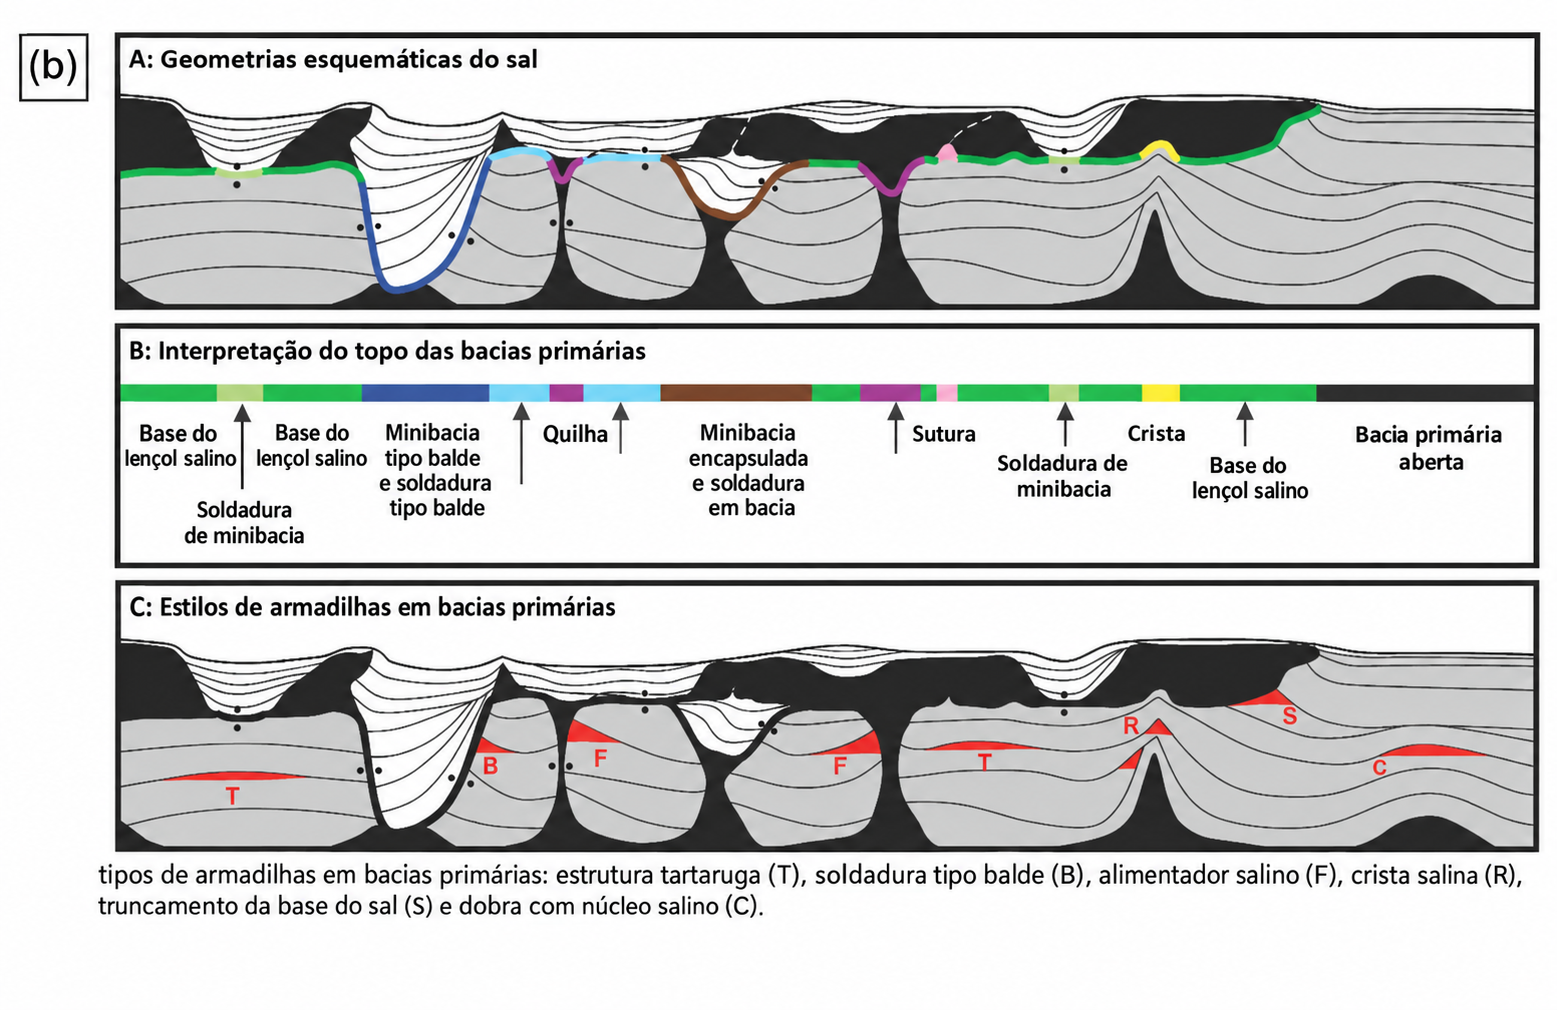
\includegraphics[width=\textwidth,height=0.78\textheight,keepaspectratio]{figuras/area-estudo/figura-20-geometrias-salinas.png}
  \caption{Geometrias salinas, superfícies de bacias primárias e estilos de armadilhas em minibacias. A tectônica salífera controla a formação de soldaduras, cristas salinas, minibacias encapsuladas e estruturas tartaruga, influenciando a distribuição de fácies e a compartimentação estrutural.}
  \label{fig:geometrias-salinas-minibacias}
  \fonte{Traduzido de \citeonline{pilcher2011}.}
\end{figure}

Na área de estudo, situada na porção norte da Bacia de Santos, próxima aos campos de Búzios e Mero, a tectônica salífera é expressa por muralhas alongadas, diápiros, altos e baixos do topo do sal, grábens de crista, falhas lístricas e minibacias pós-sal. A muralha Itapu-Búzios, por exemplo, apresenta geometria assimétrica e está associada a deformação intrassal, falhamento da cobertura e estruturas relacionadas à evacuação e ao colapso do sal. Nas proximidades de Búzios, Atapu e Mero, a geometria das minibacias demonstra que a deposição pós-sal foi fortemente condicionada pela mobilidade dos evaporitos e pelo relevo herdado da base do sal (Figura~\ref{fig:minibacia-mero}; \citeauthoronline{diorio2024}, \citeyear{diorio2024}).

\begin{figure}[htbp]
  \centering
  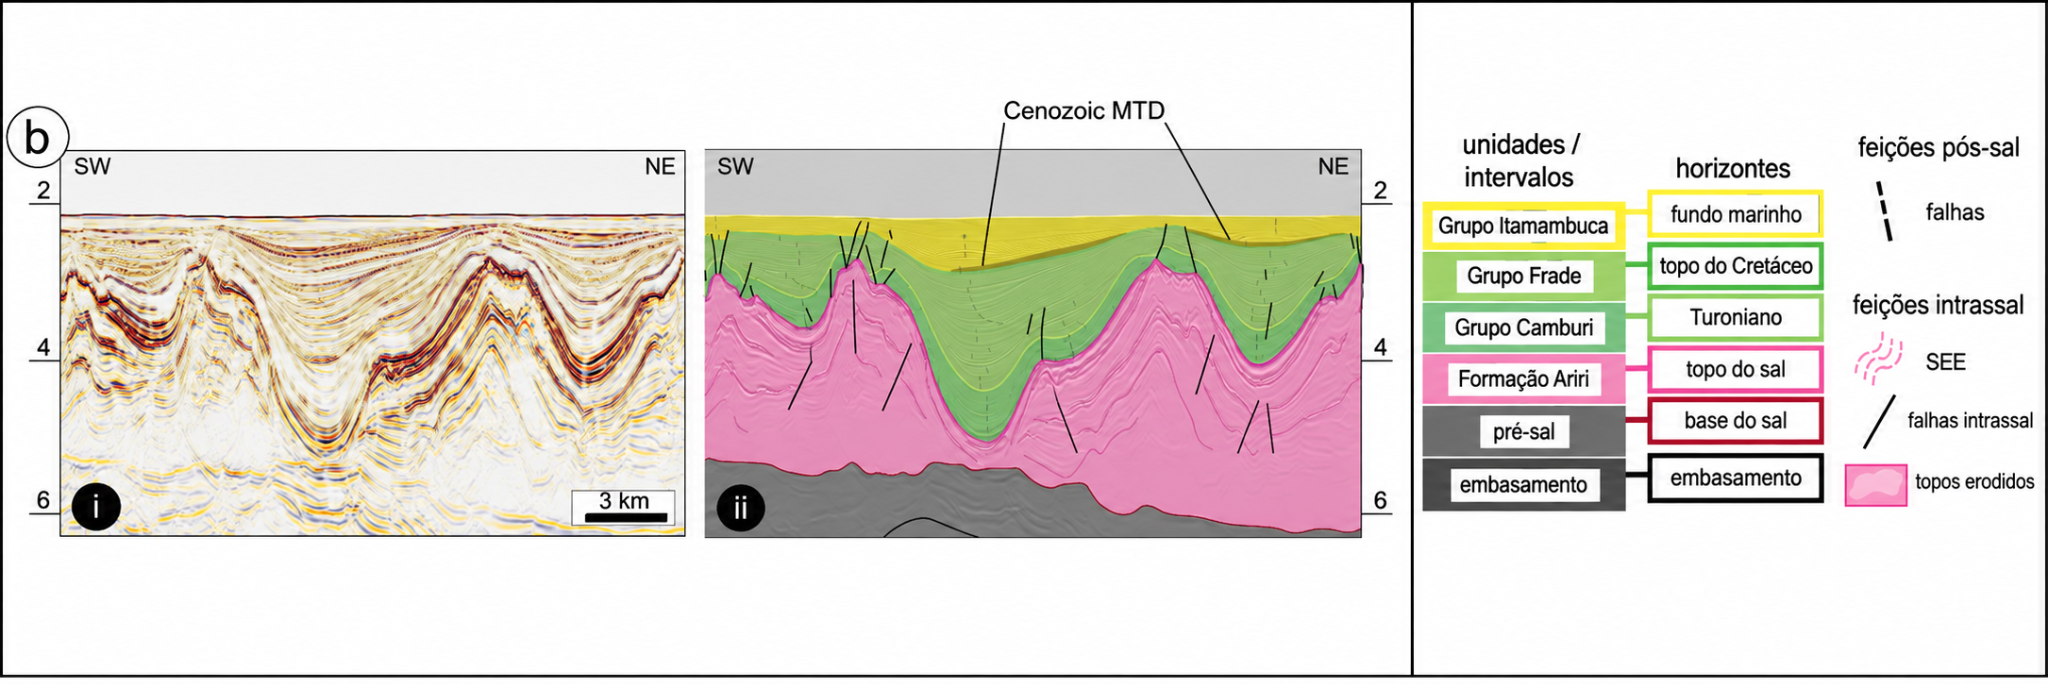
\includegraphics[width=\textwidth,height=0.78\textheight,keepaspectratio]{figuras/area-estudo/figura-21-minibacia-mero.png}
  \caption{Seção sísmica SW--NE (b) e interpretação geológica de uma minibacia do norte da Bacia de Santos, na região de Mero, destacando MTD cenozoico, falhas pós-sal e intrassal, unidades estratigráficas e a geometria da Formação Ariri. SEE: Sucessão Evaporítica Estratificada.}
  \label{fig:minibacia-mero}
  \fonte{\citeonline{diorio2024}, com tradução e reorganização da legenda.}
\end{figure}

A tectônica salífera pode atuar como importante condicionante da instabilidade do talude. A ascensão de diápiros e muralhas salinas gera relevos positivos e aumenta localmente os gradientes, enquanto a retirada de sal promove subsidência diferencial e o desenvolvimento de minibacias. A deformação da cobertura pós-sal também pode produzir arqueamentos, falhas e zonas extensionais favoráveis ao desenvolvimento de superfícies de deslizamento. Entretanto, a proximidade espacial entre um MTD e uma estrutura salina não é suficiente para atribuir à halocinese o desencadeamento da ruptura \cite{hampton1996,locat2002,masson2006}.

Além de influenciar a estabilidade do talude, a tectônica salífera pode controlar a trajetória, o confinamento e a geometria dos MTDs. Altos diapíricos e muralhas podem desviar ou limitar o deslocamento da massa, enquanto minibacias e baixos estruturais favorecem seu confinamento e acumulação. Essa interação pode produzir variações de espessura, rampas, erosão basal e diferentes padrões de deformação interna \cite{moscardelli2008,gamboa2016}. A comparação entre a geometria dos MTDs e os horizontes adjacentes permite avaliar se a relação observada corresponde principalmente a um controle morfológico da deposição ou a uma deformação que também afetou o depósito após sua formação.

\section{Canal de Santos, circulação oceânica e depósitos contorníticos}

Contornitos são depósitos formados ou retrabalhados por correntes de fundo persistentes, geralmente paralelas às isóbatas. Diferem de turbiditos e MTDs, que resultam de processos gravitacionais encosta abaixo. Na Bacia de Santos, a interação entre correntes de fundo, disponibilidade sedimentar e fisiografia do talude favoreceu o desenvolvimento do Sistema de Drift de Santos, composto por \textit{drifts}, superfícies erosivas, canais e depósitos de preenchimento \cite{rebesco2005,duarte2007}.

A circulação na porção norte da bacia é controlada principalmente pela Corrente do Brasil, pela Corrente de Contorno Intermediária e pela Corrente de Contorno Profunda, cujos sentidos de fluxo e faixas batimétricas distintas promovem erosão, transporte e deposição seletiva de sedimentos (Figura~\ref{fig:circulacao-norte-santos}) \cite{duarte2007,dutra2019,mahiques2022}. A atuação dessas correntes, associada às clinoformas eocênicas e ao relevo produzido pela tectônica salífera, condicionou a formação do Sistema de Drift de Santos e de suas feições erosivas.

\begin{figure}[htbp]
  \centering
  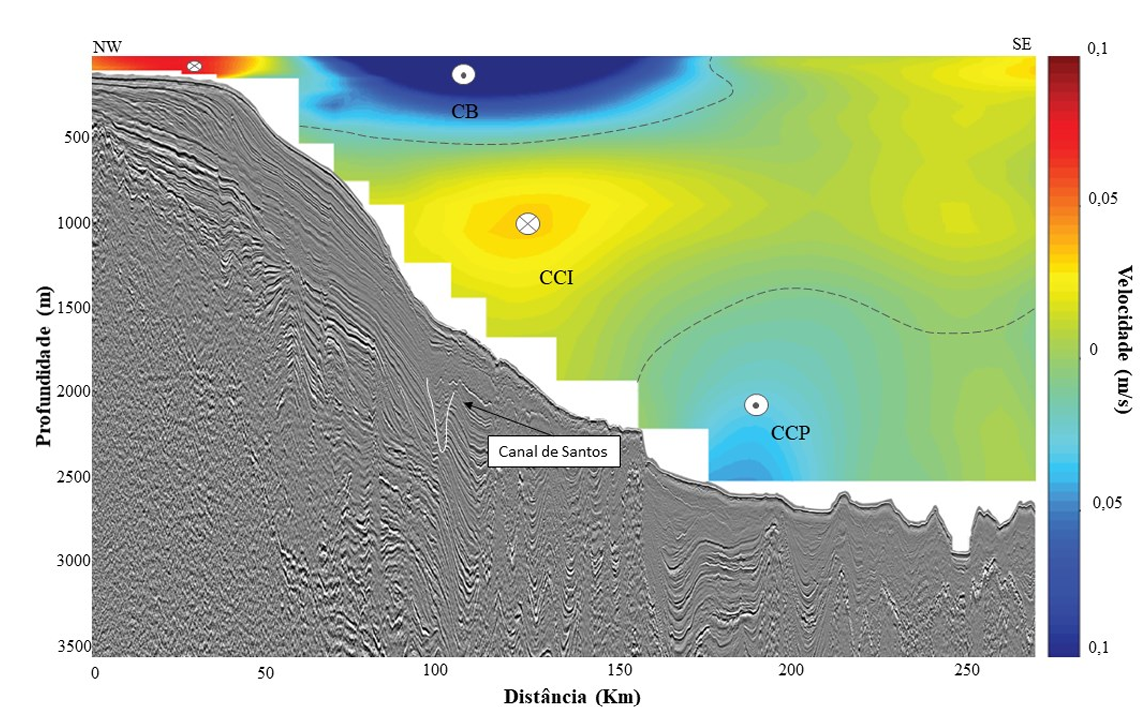
\includegraphics[width=\textwidth,height=0.78\textheight,keepaspectratio]{figuras/area-estudo/figura-22-circulacao-oceanica.png}
  \caption{Padrão de circulação oceânica no norte da Bacia de Santos. CB: Corrente do Brasil; CCI: Corrente de Contorno Intermediária; CCP: Corrente de Contorno Profunda.}
  \label{fig:circulacao-norte-santos}
  \fonte{Dados extraídos e plotados por Antônia Pamela Yhaohannah de Lima, em comunicação pessoal por meio eletrônico, conforme \citeonline{dutra2019}.}
\end{figure}

O Canal de Santos é uma importante feição erosiva desenvolvida no talude médio da porção norte da Bacia de Santos. Sua incisão ocorreu principalmente no início do Mioceno, quando correntes de fundo foram confinadas e aceleradas pela paleotopografia associada às clinoformas eocênicas. Portanto, o canal não corresponde a um canal turbidítico, embora seu preenchimento registre a interação entre processos contorníticos, gravitacionais e estruturais. Após a reorganização da margem, parte da circulação foi transferida para setores mais profundos, relacionados ao Canal de São Paulo, e o Canal de Santos passou a registrar alternâncias entre erosão, preenchimento e agradação \cite{duarte2007}.

A evolução do canal também é influenciada pela halocinese. Muralhas salinas, diápiros e minibacias modificam o espaço de acomodação e podem canalizar, acelerar ou desviar as correntes de fundo. \citeonline{dutra2019} identificou eixos de migração controlados pela fisiografia da margem e pela tectônica salífera, além de setores com redução das feições erosivas e preenchimento agradacional. A ocorrência conjunta dessas feições evidencia a interação entre processos contorníticos, gravitacionais e a deformação relacionada à tectônica salífera na evolução do Canal de Santos.
